\documentclass[12pt,a4paper]{article}
\usepackage[top=1in,bottom=1in,left=1.1in,right=1.1in]{geometry}
\usepackage{times}
\usepackage{setspace}
\usepackage{booktabs}
\usepackage{array}
\usepackage{amsmath}
\usepackage{hyperref}
\usepackage{titlesec}
\usepackage{fancyhdr}
\usepackage{parskip}
\usepackage{tabularx}
\usepackage{tikz}
\usepackage{enumitem}
\usetikzlibrary{positioning, arrows.meta, shapes.geometric,
                fit, backgrounds, calc}

\setstretch{1.25}

\hypersetup{colorlinks=true, linkcolor=black, urlcolor=black}

\titleformat{\section}{\normalsize\bfseries}{\thesection.}{0.5em}{}
\titlespacing{\section}{0pt}{12pt}{5pt}

\pagestyle{fancy}
\fancyhf{}
\lhead{\small BCSE330L -- Public Key Infrastructure and Trust Management}
\rhead{\small Case Study}
\cfoot{\thepage}
\renewcommand{\headrulewidth}{0.4pt}

\begin{document}

% ─── Header ────────────────────────────────────────────────────────
\begin{center}
{\large\bfseries Vellore Institute of Technology, Vellore}\\[0.2cm]
{\normalsize BCSE330L -- Public Key Infrastructure and Trust Management}\\[0.1cm]
{\normalsize Faculty: Dr. Berlin M A \hspace{2cm} Academic Year: 2025--26}
\end{center}
\hrule
\vspace{0.5cm}

% ─── Team Members ─────────────────────────────────────────────────
\noindent\textbf{Team Members Details:}

\vspace{0.4cm}
\begin{tabular}{p{5cm} p{6cm}}
\textbf{Reg. No} & \textbf{Name} \\[0.3cm]
23BKT0073 & Mihir Dixit \\
\end{tabular}

\vspace{0.8cm}

% ═══════════════════════════════════════════════════════════════════
\section{Title of the Project}
% ═══════════════════════════════════════════════════════════════════

\vspace{0.2cm}
\noindent\textbf{Zero-Knowledge Decentralized Public Key Infrastructure (zk-dPKI): Privacy-Preserving Certificate Management Without Centralized Certificate Authorities}

\vspace{0.8cm}

% ═══════════════════════════════════════════════════════════════════
\section{Prior Work Done}
% ═══════════════════════════════════════════════════════════════════

\vspace{0.3cm}
\renewcommand{\arraystretch}{1.5}
\begin{tabularx}{\textwidth}{|>{\centering\arraybackslash}p{2.4cm}|>{\centering\arraybackslash}p{2.8cm}|>{\centering\arraybackslash}p{2.2cm}|>{\centering\arraybackslash}X|>{\centering\arraybackslash}X|}
\hline
\textbf{\small Details of Authors} & \textbf{\small Title of the Paper} & \textbf{\small Journal / Venue} & \textbf{\small Methodology Used} & \textbf{\small Research Gap Identified} \\
\hline
Fromknecht et al.\ (2014) &
A Decentralized PKI with Identity Retention &
IACR ePrint Archive &
Name-to-key bindings stored on a Bitcoin-style chain; eliminates CAs &
On-chain storage causes chain bloat; no attribute privacy mechanism \\
\hline
Al-Bassam (2017) &
SCPKI: A Smart Contract-Based PKI and Identity System &
ACM BCC Workshop &
Certificate commitments anchored to Ethereum smart contracts; payloads off-chain &
All attributes stored in plaintext; no ZK-based selective disclosure \\
\hline
Boneh \& Franklin (2001) &
Identity-Based Encryption from the Weil Pairing &
CRYPTO 2001, LNCS &
Weil pairing on elliptic curves enables encryption from an identity string as public key &
Requires a trusted private key generator; single PKG is a trust bottleneck \\
\hline
Groth (2016) &
On the Size of Pairing-Based Non-Interactive Arguments &
EUROCRYPT 2016, LNCS &
Groth16 zk-SNARK producing 192-byte proofs via bilinear pairings on BN128 &
Trusted setup ceremony introduces toxic-waste assumption; updatable SRS needed \\
\hline
Camenisch \& Lysyanskaya (2002) &
Dynamic Accumulators and Application to Efficient Revocation &
CRYPTO 2002, LNCS &
RSA accumulator with constant-size membership and non-membership witnesses &
RSA modulus requires trusted generation; no blockchain integration for state anchoring \\
\hline
Axon \& Goldsmith (2016) &
PB-PKI: A Privacy-Aware Blockchain-Based PKI &
SECRYPT 2016 &
Dual-key architecture separating public certificate operations from identity-revealing keys &
Two-key abstraction adds management overhead; trusted authority still binds the key pair \\
\hline
Kamvar, Schlosser \& Garcia-Molina (2003) &
The EigenTrust Algorithm for Reputation Management in P2P Networks &
WWW 2003 &
Global trust scores computed as principal eigenvector of peer rating matrix via power iteration &
No mechanism for negative feedback; vulnerable to coordinated Sybil inflation attacks \\
\hline
Shamir (1979) &
How to Share a Secret &
Commun. ACM, Vol. 22 &
$(k,n)$ secret sharing over finite field via polynomial evaluation and Lagrange interpolation &
Original scheme offers no share verification; participants cannot detect incorrect shares \\
\hline
\end{tabularx}

\newpage

% ═══════════════════════════════════════════════════════════════════
\section{Summary of the Work}
% ═══════════════════════════════════════════════════════════════════

Standard Public Key Infrastructure places unconditional trust in a small number of Certificate Authorities. This arrangement has a well-documented failure mode: any CA whose private signing key is compromised can issue valid certificates for arbitrary domains, and the forged certificates are cryptographically indistinguishable from legitimate ones. The DigiNotar incident in 2011 made this consequence concrete, when attackers used a compromised CA to intercept HTTPS traffic for roughly 300,000 users. A structural fix requires removing the privileged single signing authority at the issuance layer, not auditing it more carefully.

This project replaces the CA signing authority with a threshold cryptography protocol executed by a network of validator nodes over a Byzantine Fault Tolerant consensus layer. A certificate is issued only when at least $k$ of $n$ eligible validators co-sign the certificate commitment using a Distributed Key Generation (DKG) scheme. No individual node holds a complete signing key. The certificate payload, which normally exposes the subject's full identity, is encrypted with EC-ElGamal encryption over the BN128 elliptic curve before it leaves the user's device. Validators sign a 32-byte hash commitment; they never read plaintext attributes.

At verification time, the certificate holder generates a Groth16 zero-knowledge proof that they satisfy a specific access predicate (such as holding a clearance above a threshold or belonging to a permitted role) without revealing any attribute value. The verifier calls a Solidity contract that evaluates a bilinear pairing check on BN128 and returns a boolean result. Certificate revocation replaces CRLs and OCSP with a cryptographic accumulator whose state is a single on-chain 32-byte Merkle root, making non-membership proofs constant-cost regardless of the number of revoked certificates. Private key loss is handled through Shamir's $(k,n)$ secret sharing, enabling threshold social recovery without any recovery server learning the key. Throughout, validator eligibility is enforced dynamically by an EigenRep trust scoring subsystem that continuously recomputes scores using power iteration and excludes validators whose behavior falls below a governance-defined threshold.

% ═══════════════════════════════════════════════════════════════════
\section{Objective(s) of the Work}
% ═══════════════════════════════════════════════════════════════════

\noindent\textbf{The key objectives are:}
\vspace{0.2cm}
\begin{itemize}[leftmargin=1.5em, itemsep=4pt]
    \item To eliminate single-point-of-failure certificate issuance by distributing signing authority across a $k$-of-$n$ threshold of independent validators using Distributed Key Generation (DKG), so that concurrent compromise of fewer than $k$ validators cannot produce a valid certificate.
    \item To implement attribute-level privacy in certificates using EC-ElGamal encryption over BN128, ensuring that no plaintext identity data is visible to validators, smart contracts, or ledger observers at any point in the certificate lifecycle.
    \item To enable selective attribute disclosure using Groth16 zk-SNARKs, so that a certificate holder can prove a specific claim over encrypted attributes to a verifier without revealing any other certificate field.
    \item To replace CRL and OCSP revocation with a cryptographic accumulator anchored on-chain, providing $O(1)$ non-membership proof verification regardless of the cumulative number of revoked certificates.
    \item To provide private key recovery via Shamir's $(k,n)$ Secret Sharing so that loss of the user's private key does not permanently destroy the identity binding, without any single recovery agent learning the secret.
    \item To enforce dynamic validator eligibility through EigenRep power iteration, automatically excluding validators whose trust score falls below the governance threshold within the current epoch, without a manual DAO vote.
\end{itemize}

% ═══════════════════════════════════════════════════════════════════
\section{Working Principle with Architecture Diagram}
% ═══════════════════════════════════════════════════════════════════

\subsection*{Working Principle}

The system operates across three cooperating layers. At the client layer, the user's device generates an EC-ElGamal keypair on BN128, encrypts all certificate attributes, and submits only the ciphertext and a commitment hash to the network. The private key never leaves the enclave.

At the smart contract layer, the \texttt{DAOGovernor.sol} contract receives the request, consults \texttt{TrustManager.sol} for the current EigenRep scores, and notifies only the validators above threshold. Each eligible validator computes a partial BLS signature using its DKG share. Once $k$ partial signatures are collected, the contract assembles the threshold signature, inserts the certificate's leaf hash into the accumulator tree in \texttt{AccumulatorRegistry.sol}, and emits the DID document URI. At verification time, the requester submits a 192-byte Groth16 proof and a set of public signals to \texttt{Verifier.sol}, which runs three BN128 pairing checks and returns a boolean. The accumulator root lets any relying party independently verify revocation status without querying any CA server.

\subsection*{Architecture Diagram}

\vspace{0.5cm}
\begin{center}
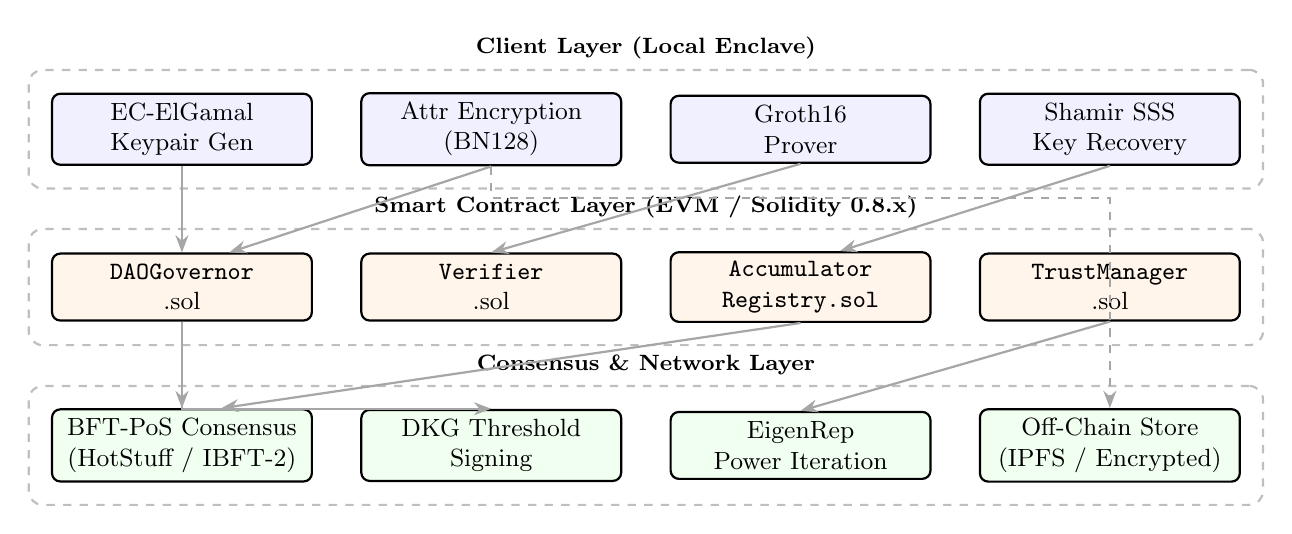
\begin{tikzpicture}[
  node distance = 0.55cm and 0.6cm,
  box/.style    = {draw, thick, rectangle, rounded corners=3pt,
                   align=center, font=\small,
                   minimum height=0.85cm},
  lbox/.style   = {box, fill=blue!6, minimum width=3.3cm},
  cbox/.style   = {box, fill=orange!8, minimum width=3.3cm},
  rbox/.style   = {box, fill=green!6, minimum width=3.3cm},
  dbox/.style   = {box, fill=gray!7,  minimum width=10.8cm},
  grp/.style    = {draw=gray!50, dashed, thick, rounded corners=5pt,
                   inner sep=8pt},
  arr/.style    = {-{Stealth[length=2.2mm]}, thick, gray!70}
]

%% ── CLIENT LAYER ──────────────────────────────────────────────────
\node[lbox] (kp)  {EC-ElGamal\\ Keypair Gen};
\node[lbox, right=of kp]  (enc) {Attr Encryption\\ (BN128)};
\node[lbox, right=of enc] (zk)  {Groth16\\ Prover};
\node[lbox, right=of zk]  (sss) {Shamir SSS\\ Key Recovery};

\begin{scope}[on background layer]
  \node[grp, fit=(kp)(enc)(zk)(sss),
        label={[font=\footnotesize\bfseries]above:Client Layer (Local Enclave)}] (client) {};
\end{scope}

%% ── SMART CONTRACT LAYER ─────────────────────────────────────────
\node[cbox, below=1.1cm of kp]  (dao)  {\texttt{DAOGovernor}\\.sol};
\node[cbox, right=of dao]       (vrf)  {\texttt{Verifier}\\.sol};
\node[cbox, right=of vrf]       (acc)  {\texttt{Accumulator}\\ \texttt{Registry.sol}};
\node[cbox, right=of acc]       (tm)   {\texttt{TrustManager}\\.sol};

\begin{scope}[on background layer]
  \node[grp, fit=(dao)(vrf)(acc)(tm),
        label={[font=\footnotesize\bfseries]above:Smart Contract Layer (EVM / Solidity 0.8.x)}] (sc) {};
\end{scope}

%% ── CONSENSUS LAYER ──────────────────────────────────────────────
\node[rbox, below=1.1cm of dao]  (bft)  {BFT-PoS Consensus\\ (HotStuff / IBFT-2)};
\node[rbox, right=of bft]        (dkg)  {DKG Threshold\\ Signing};
\node[rbox, right=of dkg]        (er)   {EigenRep\\ Power Iteration};
\node[rbox, right=of er]         (ipfs) {Off-Chain Store\\ (IPFS / Encrypted)};

\begin{scope}[on background layer]
  \node[grp, fit=(bft)(dkg)(er)(ipfs),
        label={[font=\footnotesize\bfseries]above:Consensus \& Network Layer}] (cn) {};
\end{scope}

%% ── ARROWS ───────────────────────────────────────────────────────
% client -> contracts
\draw[arr] (kp.south)  -- (dao.north);
\draw[arr] (enc.south) -- ($(dao.north)+(0.6,0)$);
\draw[arr] (zk.south)  -- (vrf.north);
\draw[arr] (sss.south) -- ($(acc.north)+(0.5,0)$);

% contracts -> consensus
\draw[arr] (dao.south) -- (bft.north);
\draw[arr] (dao.south) |- (dkg.north);
\draw[arr] (tm.south)  -- (er.north);
\draw[arr] (acc.south) -- ($(bft.north)+(0.5,0)$);

% off-chain link
\draw[arr, dashed] (enc.south) -- ++(0,-0.4) -| (ipfs.north);

\end{tikzpicture}
\end{center}

\vspace{0.3cm}
\noindent{\small \textit{Figure 1: zk-dPKI three-layer architecture. Arrows show data flow direction. Dashed line indicates off-chain encrypted payload upload. All plaintext stays in the client enclave.}}

\newpage

% ═══════════════════════════════════════════════════════════════════
\section{Novelty of the Proposed Work}
% ═══════════════════════════════════════════════════════════════════

Three aspects of this design are absent from prior published decentralized PKI systems.

\textbf{Attribute-encrypted issuance at the network layer.} Both CertCoin and SCPKI, the most cited prior works, store certificate attributes in plaintext on-chain or on IPFS. An observer who retrieves any certificate can read the subject's name, role, and organization. This design encrypts every attribute field with EC-ElGamal before the request is submitted. The validators that co-sign a certificate see only ciphertext and a commitment hash. Attribute privacy is provided by the architecture, not by access controls on a database.

\textbf{ZK proof-based access control without attribute disclosure.} Standard RBAC enforced through certificates requires the verifier to read the role field and evaluate a policy. Here, the policy is expressed as a circuit constraint, and the holder proves circuit satisfiability via a Groth16 proof. The verifier learns only whether the claim holds, not what the role or clearance value is. This makes it possible to verify access rights across multiple relying parties without any single party accumulating a profile of which claims the holder has asserted.

\textbf{Adaptive validator management through continuous trust scoring.} No prior decentralized PKI design includes a mechanism to exclude validators dynamically based on observed behavior. EigenRep recomputes the global trust vector after every observation batch. A validator that begins behaving inconsistently (equivocating in consensus, submitting implausible peer ratings) sees its score converge toward zero over the next several epochs and is excluded from the signing committee before it can accumulate enough co-signing authority to cause damage.

% ═══════════════════════════════════════════════════════════════════
\section{Key Outcomes and Results}
% ═══════════════════════════════════════════════════════════════════

The prototype implements the full certificate lifecycle in a browser application: keypair generation, EC-ElGamal attribute encryption, BFT threshold co-signing, on-chain commitment, Groth16 proof generation and on-chain verification, cryptographic accumulator revocation with non-membership proofs, and Shamir threshold key recovery. All six functional panels are wired together: revoking a certificate through the Revocation panel removes it from the ZK Proof panel's selector and updates the accumulator root displayed in the UI.

\begin{center}
\renewcommand{\arraystretch}{1.4}
\begin{tabular}{lll}
\toprule
\textbf{Operation} & \textbf{Estimated Gas} & \textbf{Complexity} \\
\midrule
Certificate issuance (commitment + threshold sig) & $\sim$142,000 & $O(k)$ partial sigs \\
Groth16 proof verification (3 BN128 pairings) & $\sim$250,000 & $O(1)$ constant \\
Accumulator update (revocation) & $\sim$65,000 & $O(\log N)$ Merkle path \\
Non-membership proof check & $\sim$45,000 & $O(\log N)$ Merkle path \\
EigenRep update (20 power iterations, 7 nodes) & Off-chain & $O(n^2 \cdot 20)$ \\
\bottomrule
\end{tabular}
\end{center}

\end{document}
